\chapter{Аналитическая часть}


\section{Явление морфинга}
Слово <<морфинг>> происходит от слова <<метаморфоза>>, которое, согласно
Согласно Оксфордскому словарю~\cite{oxford_dictionary}, имеет следующее значение: "Процесс, в ходе которого кто-то/что-то полностью превращается во что-то другое".

Таким образом, в случае трехмерных объектов термин <<морфинг>> можно интерпретировать как построение последовательности кадров, соответствующей постепенному переходу между двумя различными
объектами, так называемыми исходными (начальными) и целевыми (конечными) моделями. На рисунке~\ref{fig:morhping_example} представлен пример морфинга трехмерных объектов.

Цель морфинга заключается в вычислении преобразования, обеспечивающего визуально приятный переход между исходной и целевой формами~\cite{mocanu}. TODO: возможно здесь добавить про монотонность, сохранение точек интереса и тд (в зависимости от того, как будет работать feature preservation)

\begin{figure}[H]
    \centering
    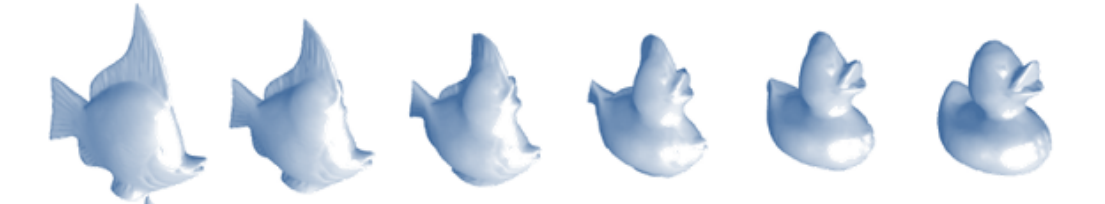
\includegraphics[width=\textwidth]{../inc/images/morhping_sequence}
    \caption{Пример последовательности кадров морфинга}
    \label{fig:morhping_example}
\end{figure}


\section{Формализация объектов сцен}

На сцене выбора начальных и конечных объектов могут присутствовать 2 фрукта: начальный и конечный. Фрукт (объект) задатся моделью описания объектов, данными для этой модели, оптическими характеристиками поверхности.

На сцене просмотра морфинга находится результат морфинга (задается исходным и целевым объектами, стадией морфинга).

На обеих сценах могут присутствовать следующие типы объектов:
\begin{itemize}
    \item источник света (задается положением в пространстве, цветом и интенсивностью света);
    \item наблюдатель (задается положением в пространстве, точкой в пространстве, на которую направлен взгляд, направлением верха обзора TODO);
\end{itemize}


\section{Выбор модели описания объекта}
Наиболее распространенные модели описания трехмерных объектов в компьютерной графике: \textit{аналитичкская}, \textit{полигональная модель}, \textit{воксельная модель}~\cite{porev}.

\subsection{Аналитическая модель}
Аналитическая модель представляет собой описание поверхности математическими формулами~\cite{porev}. Обычно поверхность задается уравнением вида $z=f(x,y)$ или $F(x,y,z)=0$.

Отличительные черты~\cite{porev}:
\begin{itemize}
    \item легкая процедура рассчета координат точек, нормалей;
    \item небольшой объем информации для описания форм;
    \item сложные формулы, которые медленно вычисляются компьютером;

    % TODO: Начиная отсюда идет отсебятина, а не источник, это номр???
    \item задание объекта набором поверхностей, если невозможно описать его аналитически;
    \item отсутствие погрешности при задании сферического объекта;
\end{itemize}

\subsection{Полигональная модель}
В полигональной модели информация об объекте сосотоит из следущих компонентов~\cite{porev}:
\begin{itemize}
    \item вершина --- точка ($(x, y, z)$ в декартовой системе координат);
    \item отрезок прямой --- задается двумя вершинами;
    \item полилиня --- задается несколькими отрезками прямой;
    \item полигон --- описывает плоскую грань объемного объекта в виде замкнутой линии;

    Несколько граней (полигонов) составляют объемный объект в виде полигональной поверхности, также назваемой <<полигональной сеткой>>.
\end{itemize}

\subsection{Воксельная модель}
TODO

\subsection{Сравнение моделей описания объектов}
TODO: а надо ли мне вообще выбирать, если у меня в ТЗ написанно НИЗКОПОЛИГОНАЛЬНЫЕ ОБЪЕКТЫ????
TODO: можно сравнить по критериям: сложность вычисления нормали, изображение любых объектов, сохранение качества при увеличении

Среди всех моделей наиболее подходящей является полигональная модель, т.~к. с помощью нее можно описать объекты любой сложности, и сохраняет качестве при увеличении, что необходимо в задаче интерактивной визуализации морфинга,  поэтому использованная будет именно она.


\section{Основные этапы морфинга}

\subsection{Установление соответствия между объектами}
3D‑сетки часто различаются по топологии (число вершин/граней и связность), поэтому прямое сопоставление поверхностей затруднено. Соответствие получают косвенно через \textit{параметризацию} — биективное отображение поверхности сетки в общую параметрическую область $D$, обычно единичный диск для незамкнутых сеток (\textit{плоская парамеризация}) или единичная сфера для замкнутых (\textit{сферическая параметризация})~\cite{mocanu}.

Сферическая параметризация примяется к замкнутым поверхностям нулевого рода~\cite{mocanu}, или не имеющим отверстий, коими являются фрукты в рамках данной работы.

\subsection{Параметризация}

Выделяют 3 основных подхода к параметризации сеток: \textit{плоская}, \textit{сферическая}, \textit{разбиение на участи с плоской параметризацией} \cite{mocanu,alexa}.

Плоская праметризация применима для незамкнутых сеток~\cite{mocanu,alexa}, поэтому она непригодна для морфинга замкнутных объектов, таких, как фрукты.

Если исходный и целевой объекты имеют существенно различающиеся формы или представляют собой поверхности разного рода, т.~е. имеют разное число отверстий, применяют предварительное разбиение на плоские участки \cite{mocanu}. Пользователь вручную разбивает исходную и целевую сетки на участки и задаёт их соответствие; затем для каждого участка выполняется плоская параметризация. Данный метод требует значительного участия пользователя, от которого зависит качество результата, поэтому в настоящей работе он не рассматривается.

%\subsection{Параметризация звездообразных тел}
%\textit{Звездообразным} называется тело, которое имеет хотябы одну внутреннюю точку такую, что отрезки, соединяющие ее с вершинами тела, полностью лежат внутри фигуры \cite{alexa}.

%Пусть точка $O$ видна из всех вершин тела $A$. Тогда, чтобы параметризовать тело $A$, необходимо перенесити его так, чтобы точка $O$ совпала с началом координат и нормировать координаты всех вершин.

%\subsection{Метод релаксации}
Для сферической параметризации произвольных поверхностей нулевого рода, применяется метод релаксации, основаный на итеративном уточнении положений вершин~\cite{alexa}. Процесс релаксации сетки представлен на рисунке~\ref{fig:relaxation}.

В качестве начального состояния строят грубую проекцию сетки на единичную сферу: выбирают любую внутреннюю точку модели в качестве центра сферы и проецируют все вершины на её поверхность (нормализуют радиус‑векторы). Полученная начальная конфигурация обычно содержит значительные искажения и грани с неправильной ориентацией. Процесс релаксации продолжают до тех пор, пока все грани не приобретут корректную ориентацию — внешняя сторона каждой грани должна быть обращённой наружу сферы~\cite{alexa}.

На каждом раунде релаксации вершины сдвигаются к центру масс своих соседей:

\begin{equation}
    v_i^{k + 1} = \frac{\sum_{j \in N(i)} v_j^{k}}{\parallel \sum_{j \in N(i)} v_j^{k} \parallel},
\end{equation}

где
\begin{itemize}
    \item $v_i^{k + 1}$ --- положение $i$-ой вершины после $k$-го раунда релаксации;
    \item $v_i^{k}$ --- положение $i$-ой вершины на момент $k$-го раунда релаксации;
    \item $N(i)$ --- множество вершин, смежных с $i$-ой.
\end{itemize}

Для предотвращения коллапса всех вершин в одну точку после каждой итерации выполняется ре-центрирование всей сетки относительно начала координат~\cite{alexa}:

\begin{equation}
    v_i' = v_i - \frac{\sum_{j = 0}^{n} v_j}{n},
\end{equation}

где
\begin{itemize}
    \item $v_i'$ --- новое положение $i$-ой вершины;
    \item $n$ --- количество вершин.
\end{itemize}

\begin{figure}[H]
    \centering
    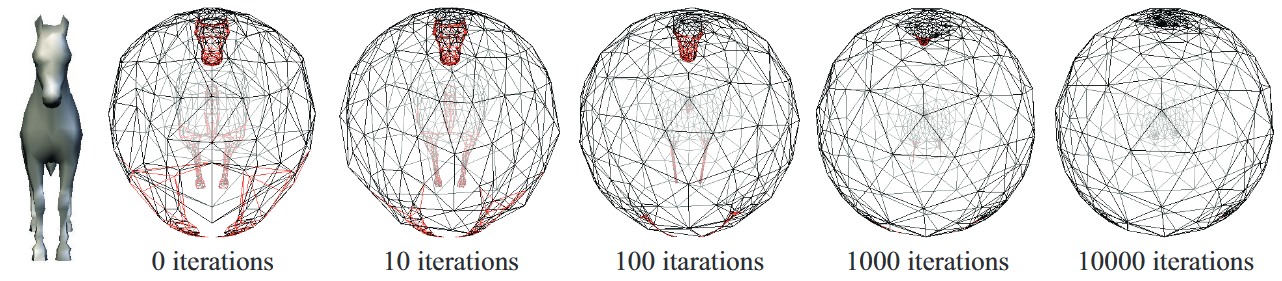
\includegraphics[width=\textwidth]{../inc/images/relaxation}
    \caption{Процесс релаксации сетки, красными отмечены грани c непрвильной ориентацией}
    \label{fig:relaxation}
\end{figure}

\subsection{Создание общего представления}
После того как установлено соответствие, необходимо создать единую структуру, которая будет использоваться для всех промежуточных форм. Обычно для этого сроят \textit{суперсетку} --- сетку, содержащую вершины исходной и целевой сетки, а также их точки пересечения~\cite{mocanu,alexa} (пример на рисунке~\ref{fig:supermesh}).

На параметрической сфере сетки накладываются друг на друга; в местах пересечения ребер создаются новые вершины, что формирует объединенную сетку, которая может принимать форму, как исходной так и целевой модели; поскольку полученная сетка обычно не является треугольной, выполняют её треангуляцию. Для этого используется треангуляция Делоне, поскольку она минимизирует количество узких треугольников, что улучшает качество сетки~\cite{mocanu,alexa}.

\begin{figure}[H]
    \centering
    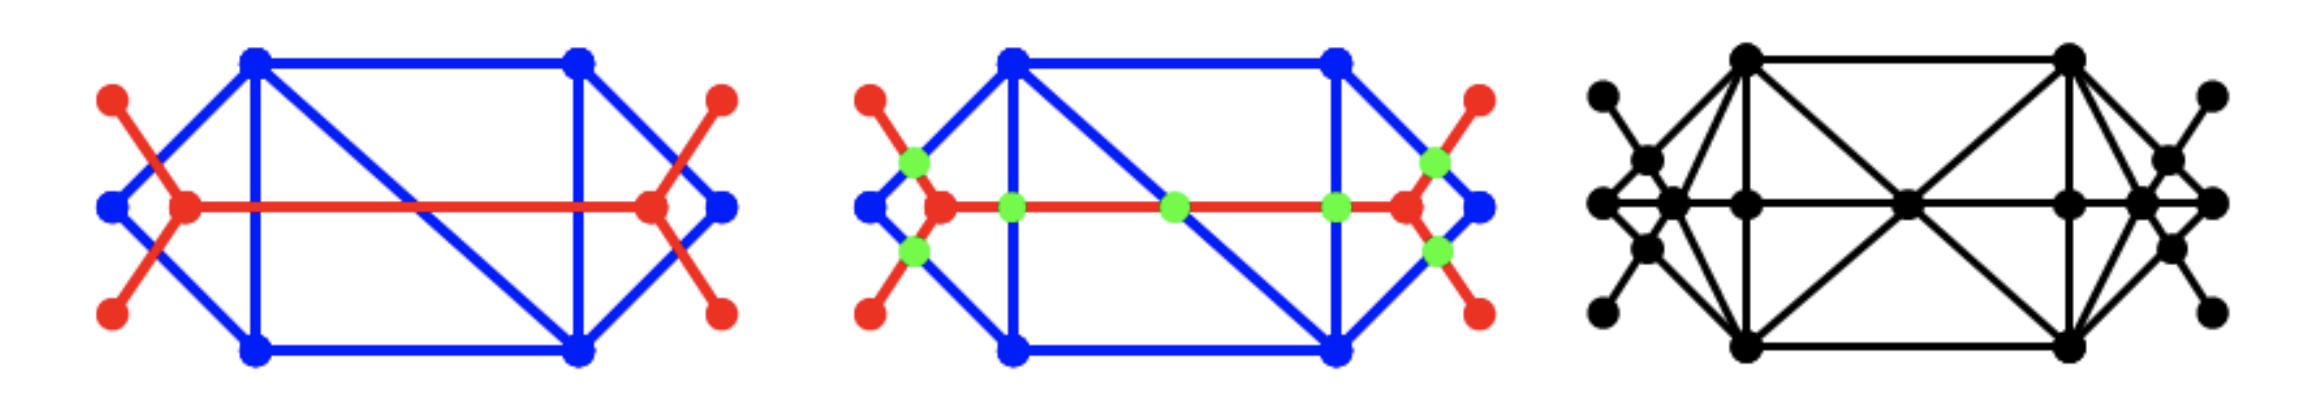
\includegraphics[width=\textwidth]{../inc/images/supermesh}
    \caption{Создание суперсетки}
    \label{fig:supermesh}
\end{figure}

\subsection{Интерполяция геометрии}
Заключительный этап --- вычисление траекторий движения вершин общего представления из их начальных положений до конечных. Для каждой вершины суперсетки необходимо определить ее координаты на исходной и целевой моделях. Процесс генерации промежуточных кадров сводится к интерполяции этих координат.

Положение вершины на каждой из моделей определяется с помощью барицентрических координат в параметрическом пространстве\cite{mocanu,alexa}. Алгоритм сводится к следующим шагам:

Процесс вычисления состоит из следующих шагов:
\begin{enumerate}
    \item[1)] Поиск содержащего треугольника: Для каждой определяется треугольник исходной (или целевой) сетки, в который она попадает в общем параметрическом пространстве (на сфере).
    \item[2)] Вычисление барицентрических координат данной вершины относительно вершин найденного треугольника.
    \item[3)] Барицентрические координаты применяются к вершинам соответствующего треугольника в мировых координатах.
\end{enumerate}

После получения начальных и конечных положений $P0$ и $P1$ для каждой вершины траектории генерируют посредством линейной интерполяции~\cite{mocanu,alexa}. Положение вершины в момент времени $t\in [0,1]$ вычисляется по формуле~\eqref{eq:lerp}.

\begin{equation}
    \label{eq:lerp}
    P(t) = (1 - t) \cdot P_0 + t \cdot P_1
\end{equation}

TODO: добавить про интерполяцию материала и нормалей


\section{Анализ алгоритмов удаления невидимых линий и поверхностей}

Алгоритмы удаления невидимых линий и поверхностей служат для удаления ребер, поверхностей или объемов, которые видимы или невидимы для наблюдателя, находящегося в заданной точке пространства\cite{rogers}.

Рассмотрим следующие алгоритмы: \textit{алгоритм Робертса}, \textit{алгоритм, использоующий z-буфер}, \textit{алгоритм трассировки лучей}.

\subsection{Алгоритм Робертса}

Данный алгоритм применим только к выпуклым телам. Если обрабатываемое тало невыпуклое --- его необходимо предварительно разбить на выпуклые~\cite{rogers}.

Алгоритм состоит из следующих этапов~\cite{rogers}:
\begin{enumerate}
    \item[1)] Удаление граней, экранируемых самим телом.
    \item[2)] Удаление граней, экранируемых другими телами.
    \item[3)] Удаление линий пересечения тел, экранируемых самими телами.
\end{enumerate}

Ассимптотическая оценка трудоемкости: $O(N^2)$, где $N$ --- количество граней. TODO: проверить

\subsection{Алгоритм, использующий \textit{z}-буфер}

Идея \textit{z}-буфера является обобщением идеи буфера кадра. Буфер кадра используется для запоминания аттрибутов (интенсивности) каждого пикселя в пространстве изображения. \textit{z}-буфер --- это отдельны буфер глубины, используемый для запоминания координаты \textit{z} каждого видимого пикселя в пространстве изображения\cite{rogers}.

Этапы работы алгоритма~\cite{rogers}:

\begin{enumerate}
    \item[1)] Заполнить буфер кадра фоновым значением.
    \item[2)] Заполнить z-буфер минимальным значением глубины.
    \item[3)] Выполнить переход в пространство изображения.
    \item[4)] Для каждого пикселя ($x$, $y$), пренадлежащего телу вычислить его глубину $z(x, y)$.
    \item[5)] Если глубина $z(x, y)$ > $z\textit{-буфер}(x, y)$, то записать атрибут текущего тела в $\textit{буфер-кадра}(x, y)$, записать глубину $z(x, y)$ в $z\textit{-буфер}(x, y)$.
\end{enumerate}


Асимптотическая оценка трудоекости: $O(N)$, где $N$ --- количество граней. TODO: проверить

\subsection{Алгоритм художника}

Идея алгоритма состоит в том, чтобы подобно художнику отрисовывать объекты по мере их приближения к наблюдателю.

Основные этапы алгорима~\cite{rogers}:
\begin{enumerate}
    \item[1)] Отсортировать грани по минимальному или максимальному значению глубины.
    \item[2)] Отрисовать грани в отсортированном порядке.
\end{enumerate}

Простая сортировка не всегда дает корректный список приоритетов, тогда приходится использовать дополнительные методы разрешения конфликтов~\cite{rogers}.

Алгоитм не справляется со случаями циклического перекрытия и пересечения многоугольников.

Ассиптотическая оценка трудоемкости: $O(N)$, где $N$ --- количество граней, однако стоит дополнительно учитывать трудоемкость предварительной сортировки.

\subsubsection{Алгоритм трассировки лучей}
Идея метода заключается в том, что наблюдатель видит любой объект посредством испускаемого неким источником света, который падает на этот объект и некоторомы путем доходит до наблюдателя. Однако обычно используют алгоритм обратной трассировки лучей, в котором лучи пускаются от наблюдателя~\cite{rogers}.

Полагая, что объекты сцены уже находятся в простратсве изображения, выполняются следующие этапы для каждого пикселя~\cite{rogers}:

\begin{enumerate}
    \item[1)] Составить уравнение отслеживаемого луча.
    \item[2)] Найти пересечение луча со всеми гранями.
    \item[3)] Среди всех пересечений найти ближайшее к наблюдатею и использовать аттрибуты объекта, которому соответвствует пересечение для определения цвета пикселя. Если пересечений нет --- закрасить пиксель цветом фона.
\end{enumerate}

Ассимптотическая оценка трудоемкости: $O(WHN)$, где $W$ --- ширина экрана в пикселях, $H$ --- высота экрана в пикселях, $N$ --- количество граней.

\subsection{Сравнение алгоритмов}

В таблице~\ref{tbl:invisible_faces_removal_comparison} представленные результаты сравнения алгоритмов и использованы следующией обозначения:

\begin{itemize}
    \item Р --- алгоритм Робертса;
    \item ZБ --- алгоритм, использующий \textit{z}-буфер;
    \item Х --- алгоритм Художника;
    \item ТЛ --- алгоритм трассировки лучей.
\end{itemize}


\begin{table}[H]
    \centering
    \caption{Сравнение алгоритмов удаления невидимых линий и поверхностей}
    \label{tbl:invisible_faces_removal_comparison}
    % Определяем новый тип столбца C для центрирования в ячейке с заданной шириной и по вертикали
    \newcolumntype{C}[1]{>{\centering\arraybackslash}m{#1}}
    \newcolumntype{J}[1]{>{\justifying\arraybackslash}m{#1}}

    % Ширина первого столбца ~35% от ширины текста
    % Ширина остальных 6 столбцов ~10.8% каждая
    \begin{tabular}{|p{0.35\textwidth}|C{0.13\textwidth}|C{0.13\textwidth}|C{0.13\textwidth}|C{0.13\textwidth}|}
        \hline                                  & \textbf{Р} & \textbf{ZБ} & \textbf{Х} & \textbf{ТЛ} \\
        \hline
        Совместимость с любыми телами            & -          & +           & +          & +           \\
        \hline
        Возможность использования без сортировки & +          & +           & -          & +           \\
        \hline
        Возможность учета прозрачности           & -          & +           & +          & +           \\
        \hline
        Асиптотическая оценка трудоемкости       & $O(N^2)$   & $O(N)$      & $O(N)$     & $O(WHN)$    \\
        \hline
    \end{tabular}
\end{table}

Среди всех расмотренных алгоритмов, алгоритм, использующий \textit{z}-буфер подходит больше остальных, т.~к. он имеет лучшую асимптотическую оценку трудоемкости и применим к любым телам, что необходимо при решении задачи визуализации морфинга.


\section{Модель освещения}

В компьютерной графике наиболее распространненными являются две модели освещения: \textit{локальная} и \textit{глобальная}~\cite{rogers}.

Локальная модель учитывает только свет, падающий от источника (источников), и ориентацию поверхности~\cite{rogers}.

Глобальная модель освещения учитывает также свет, отраженный от других объектов сцены или пропущенный через них~\cite{rogers}.

Поскольку на сцене будет находиться только один объект, то будет использована локальная модель освещения.

Интенсивность $I$ в точке $P$ в локальной модели вычисляется по формуле~\eqref{eq:local_light_model}~\cite{rogers}.

\begin{equation}
    \label{eq:local_light_model}
    I = k_aI_a + \frac{I_l}{d + K}[k_d(\mathbf{\hat{n}\cdot \hat{L}})+k_s(\mathbf{\hat{R}\cdot \hat{S}})^\alpha],
\end{equation}

где \\
$k_a$ --- коэффициент TODO; \\
$I_a$ --- интенсивность фонового освещения; \\
$I_l$ --- интенсивность источника света; \\
$d$ --- расстояние от источника света до точки~$P$; \\
$K$ --- добавка уменьшения интенсивности света с расстоянием (выбирается из эстетических предпочтений); \\
$k_d$ --- коэффициент диффузного отражения поверхности; \\
$\mathbf{n}$ --- вектор нормали к поверхности в точке $P$; \\
$\mathbf{L}$ --- вектор, обратный вектору падения луча; \\
$k_s$ --- коэффициент зеркального отражения поверхности; \\
$\mathbf{R}$ --- вектор, отраженного луча; \\
$\mathbf{S}$ --- вектор, направленный на наблюдателя из точки $P$; \\
$\alpha$ --- степень, аппроксимирующая пространственное распределение зеркально отраженного света.


\section{Анализ алгоритмов закраски}

Основными алгоритмами закраски в комьютерной графике являются: \textit{однотонная закраска}, \textit{закраска методом Гуро}, \textit{закраска методом Фонга}~\cite{rogers}.

\subsection{Однотонная закраска}
При однотонной закраске для каждой грани (многоугольника) полигональной поверхности вычисляется один уровень интенсивности, с которым закрашивается вся гранть. В результате такой закраски изображенный состоит из отдельных иногоугольников и объект выглядит, как многогранник~\cite{rogers}.

\subsection{Закраска методом Гуро}
Этот метод предназначен для создания иллюзии гладкой криволинейной поверхности, описанной в виде многогранников или полигональной сетки с плоскиими гранями\cite{rogers,porev,foley}

Метод Гуро основан на интерполяции интенсивности каждого пикселя при закраске. Закрашивание граней по методу гуро осуществляется в четыре этапа~\cite{porev}:

\begin{enumerate}
    \item [1)] Определение нормали к каждой грани.
    \item [2)] Определение нормалей в вершинах путем усреднения нормалей прилежащих граней.
    \item [3)] На основе нормалей в вершинах вычисляются значения интенсивностей в вершинах согласно выбранной модели освещения.
    \item [4)] Закрашиваются полигоны граней цветом, соответствующим интерполяции значений интенсивности в вершинах.
\end{enumerate}

\subsection{Закраска методом Фонга}

Аналогичен методу Гуро, но при использовании метода Фонга для определения цвета в каждой точке интерполируются не интенсивности отраженного света, а векторы нормалей. При этом значение интенсивность вычисляется в каждом внутреннем пикселе грани~\cite{rogers,porev}.

\subsection{Сравнение алгоритмов закраски}

Визуальное сравнение алгоитмов представленно на рисунке~\ref{fig:shading_comparison}.

\begin{figure}[H]
    \centering
    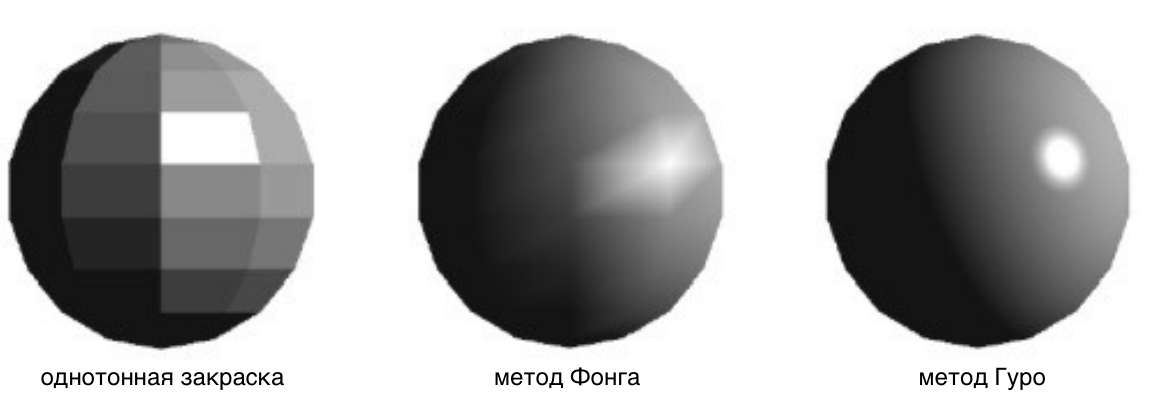
\includegraphics[width=1\textwidth]{../inc/images/shading_2}
    \caption{Визуальное сравнение методов закрски}
    \label{fig:shading_comparison}
\end{figure}

Поскольку объекты сцены (фрукты) представлены низкополигональными объектами, предпочтительной является однотонная закраски, обеспечивающая дискретность освещения между смежными гранями. В результате мофринга часто возникает множество полигонов, составляющих одну грань, из-за чего при однотонной закраске возникают световые артефакты, как на рисунке~\ref{fig:gouraund_midified},~a.

Для устранения этой проблемы будет использована модифицированная версия закраски Гуро: значение интенсивности вершин в пределах одной грани вычисляется с помощью нормали к этой грани, а не нормалей в вершинах. Это обеспечивает равномерное распределение интенсивности по грани и предотвращает сглаживание рёбер, что продемонстрированно на рисунке~\ref{fig:gouraund_midified},~б.

\begin{figure}[H]
    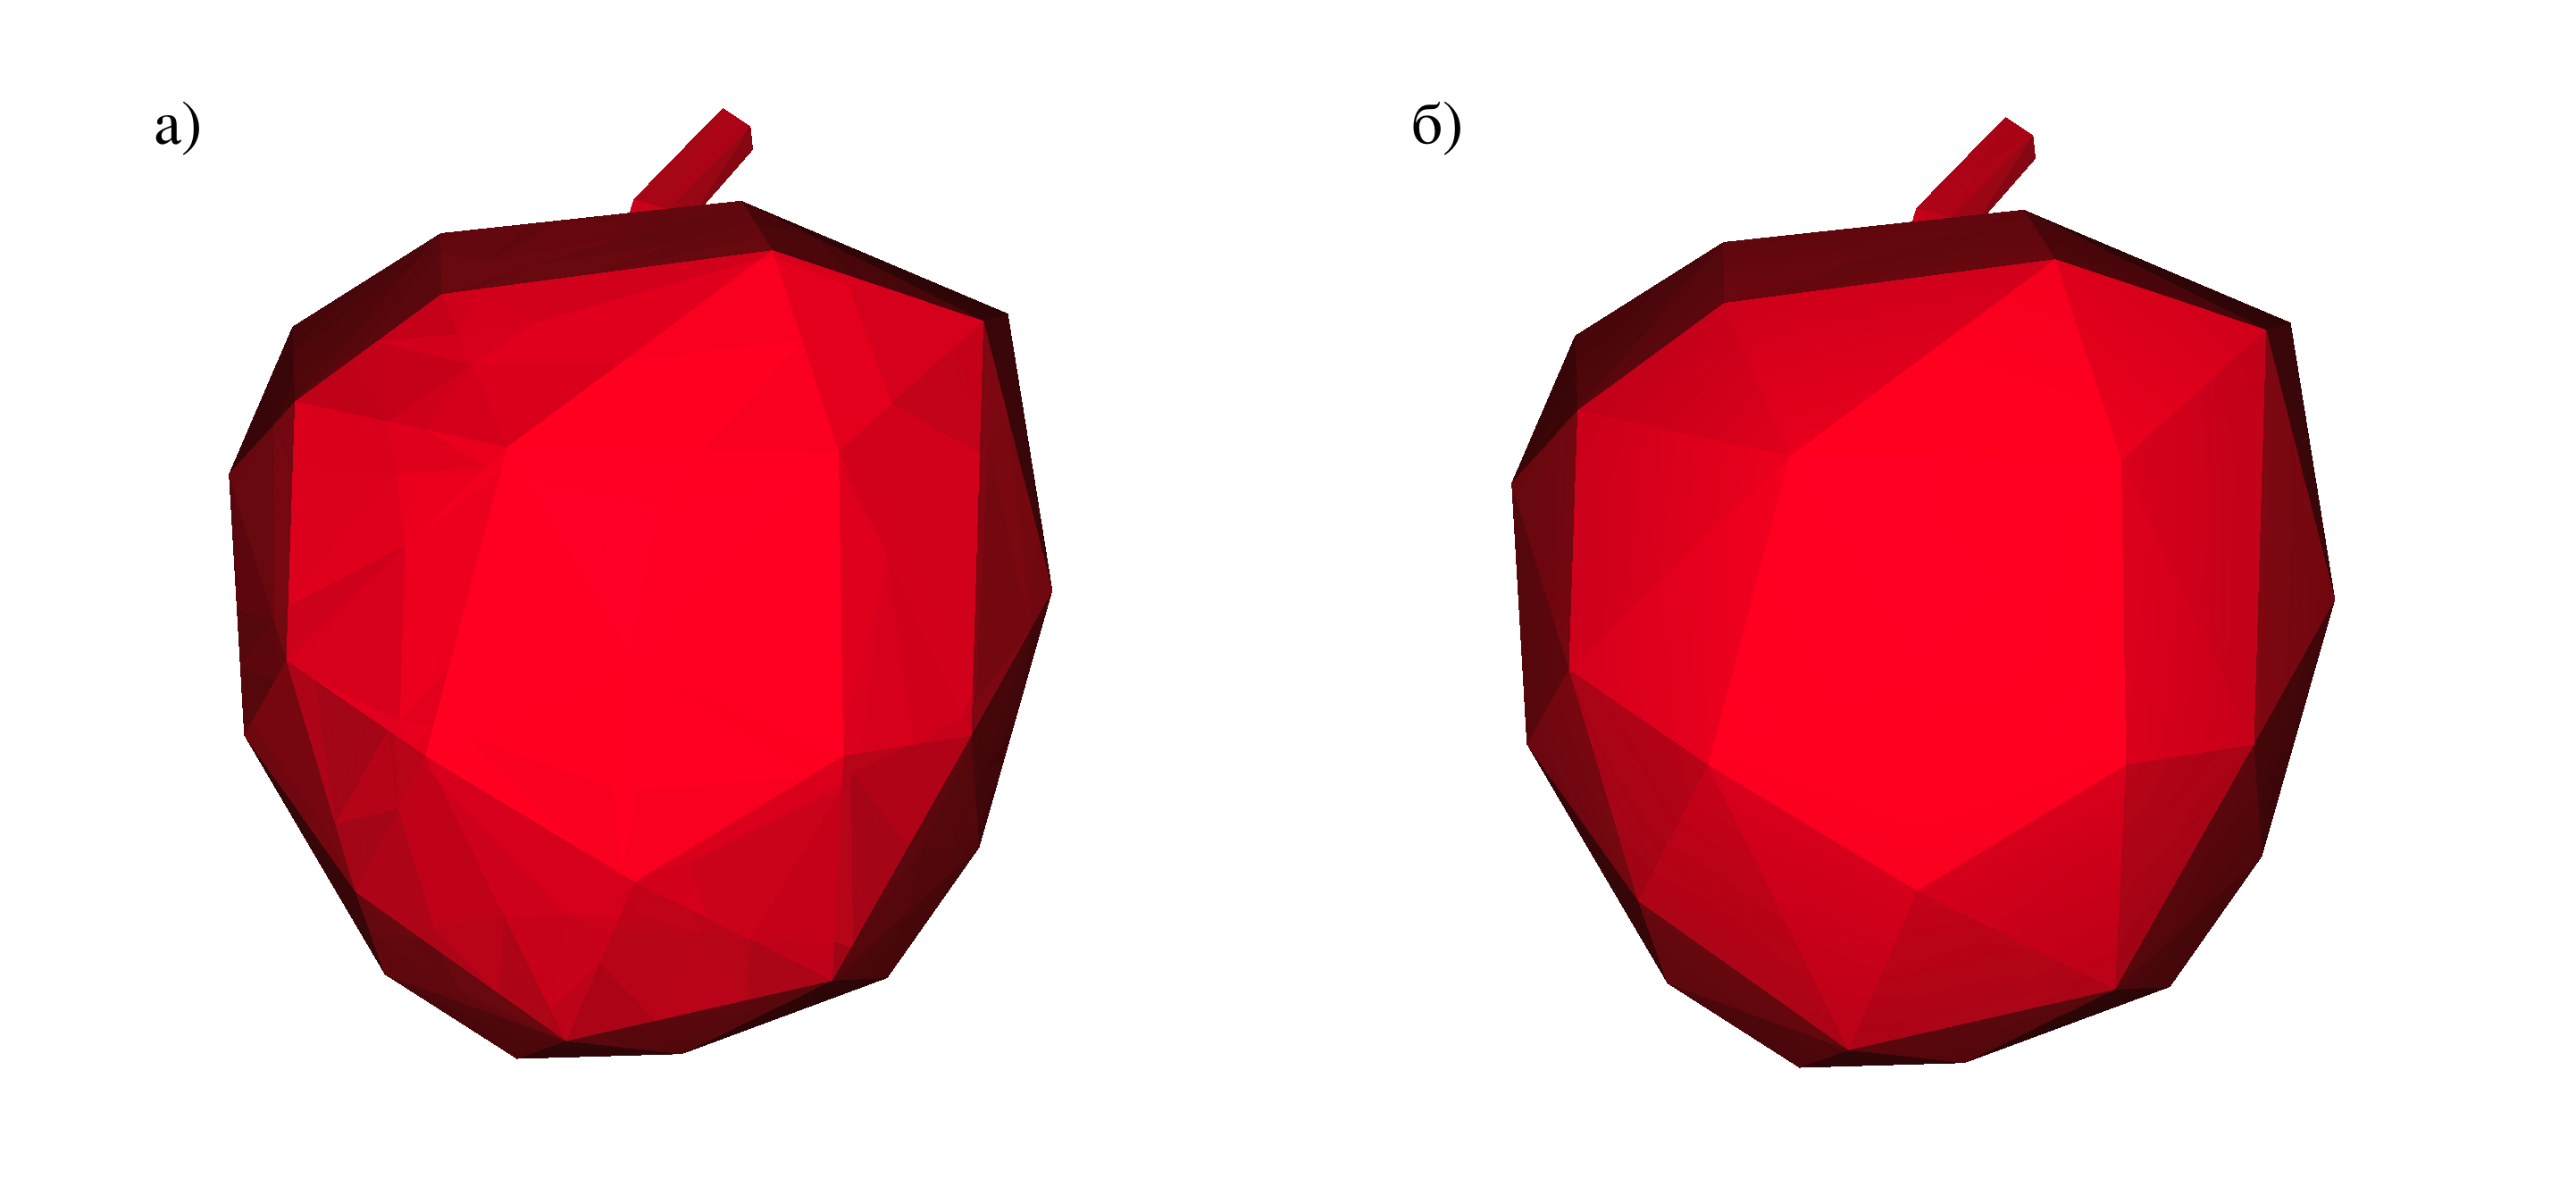
\includegraphics[width=\linewidth]{../inc/images/gouraund_modified}
    \caption{Результат морфинга с использованием различных алгоритмов закраски: а) однотонная закраска; б) закраска модифицированным методом Гуро}
    \label{fig:gouraund_midified}
\end{figure}


\section*{Вывод}

В аналитической части были рассмотрены основные этапы морфинга, проанализированны модели представления объектов и алгоритмы решения основных задач компьютерной графики. По результатам проведенного анализа были выбраны: полигональное представление модели, алгоритм, использющий ~\textit{z}-буфер для удаления невидимых линий и поверхностей, простая модель освещения, модифиицированная закраска Гуро.


\clearpage